\documentclass[11pt]{article}
\usepackage[margin=1in]{geometry}
\usepackage{graphicx}
\usepackage{booktabs}
\usepackage{amsmath}
\usepackage{caption}
\usepackage{float}
\usepackage[numbers,sort&compress]{natbib}
\usepackage[colorlinks=true,linkcolor=black,citecolor=blue,urlcolor=blue]{hyperref}

\graphicspath{{../figures/}}
\captionsetup{font=small,labelfont=bf}
\setlength{\parskip}{2pt}

\title{\vspace{-1.5em}Multi-Timescale Volatility Forecasting:\\
Transferring a Dual-Resolution TCNN-LSTM from Human Activity Recognition}
\author{Mohamed Diallo\\
\small IE412 AI for Finance, UNIST, Spring 2026}
\date{June 2026}

\begin{document}
\maketitle

\begin{abstract}
\noindent
Realized-volatility forecasting and the heterogeneous autoregressive (HAR-RV) model of
\citet{corsi2009} rest on a multi-timescale prior: volatility is best predicted by combining
information aggregated over a day, a week, and a month. We observe that this prior is
structurally identical to a dual-resolution hybrid TCNN-LSTM that we recently co-proposed for
human activity recognition \citep{warnants2026}, which fuses a short-context and a long-context
branch. This project transfers that architecture to one-day-ahead volatility forecasting for the
S\&P~500 and compares it against GARCH(1,1) and HAR-RV using RMSE, the QLIKE loss, and
Diebold-Mariano tests. On the 2021--2026 test set the transferred model attains the lowest
squared-error loss and significantly improves on HAR-RV (Diebold-Mariano $p=0.013$); a five-seed
robustness sweep confirms the improvement is stable, and a branch ablation confirms the
dual-resolution design contributes. The gain is small in absolute terms because the daily
volatility proxy is intrinsically noisy, which we analyze explicitly. The contribution is a clear
logical link from a known financial inductive bias to a learned architecture that respects it.
\end{abstract}

\section{Introduction and Motivation}
Volatility is the central input to risk management, option pricing, and portfolio construction,
and forecasting it one day ahead is a canonical problem in financial econometrics. The dominant
practical model, the heterogeneous autoregressive model of realized volatility (HAR-RV)
\citep{corsi2009}, is deceptively simple: it predicts tomorrow's log realized variance as a linear
combination of the most recent daily value, the trailing weekly average, and the trailing monthly
average. Its effectiveness comes from an explicit \emph{multi-timescale} inductive bias, the
heterogeneous-market hypothesis that traders operating at different horizons each leave a footprint
in volatility.

The motivation for this project is an observation that this inductive bias is not unique to
finance. In recent co-authored work on human activity recognition (HAR) for ambient-assisted living
\citep{warnants2026}, we proposed a hybrid temporal-convolutional LSTM that processes a short-context
window (two minutes, capturing brief actions) and a long-context window (two hours, capturing extended
routines) on two parallel branches before fusing them. The structural correspondence is exact:
HAR-RV's daily, weekly, and monthly aggregates are a fixed, hand-engineered version of the same
short-versus-long multi-resolution decomposition that the deep model learns. This paper asks whether
transferring that architecture, with its information set held equal to HAR-RV's, improves volatility
forecasts, and whether any improvement is statistically real rather than an artifact of a single
training run. We frame prediction quality with both a statistical loss and a robustness analysis,
and we are explicit about the limits imposed by the data.

\section{Related Work and the HAR Analogy}
HAR-RV \citep{corsi2009} approximates the long-memory dynamics of realized variance with three lag
aggregates and remains a strong baseline that newer models are routinely measured against. GARCH
\citep{bollerslev1986} models the conditional variance of returns directly and is the classical
benchmark. On the deep-learning side, recurrent and convolutional models have been applied to
volatility, but they rarely make their multi-timescale prior explicit.

Our prior HAR architecture \citep{warnants2026} makes that prior its central design choice. It uses
two parallel sliding windows, a two-minute short-term window and a two-hour long-term window, each
processed by temporal convolutional layers with dilated convolutions that expand the receptive field
without inflating the parameter count, and fuses the two branches through a recurrent step. Figure
\ref{fig:analogy} places the two designs side by side: HAR-RV fixes the timescales and the linear
weights a priori, whereas the dual-resolution TCNN-LSTM learns convolutional features over the same
short and long horizons. This paper treats the deep model as a learned generalization of HAR-RV and
tests whether the added flexibility pays off at the daily horizon.

\begin{figure}[H]
\centering
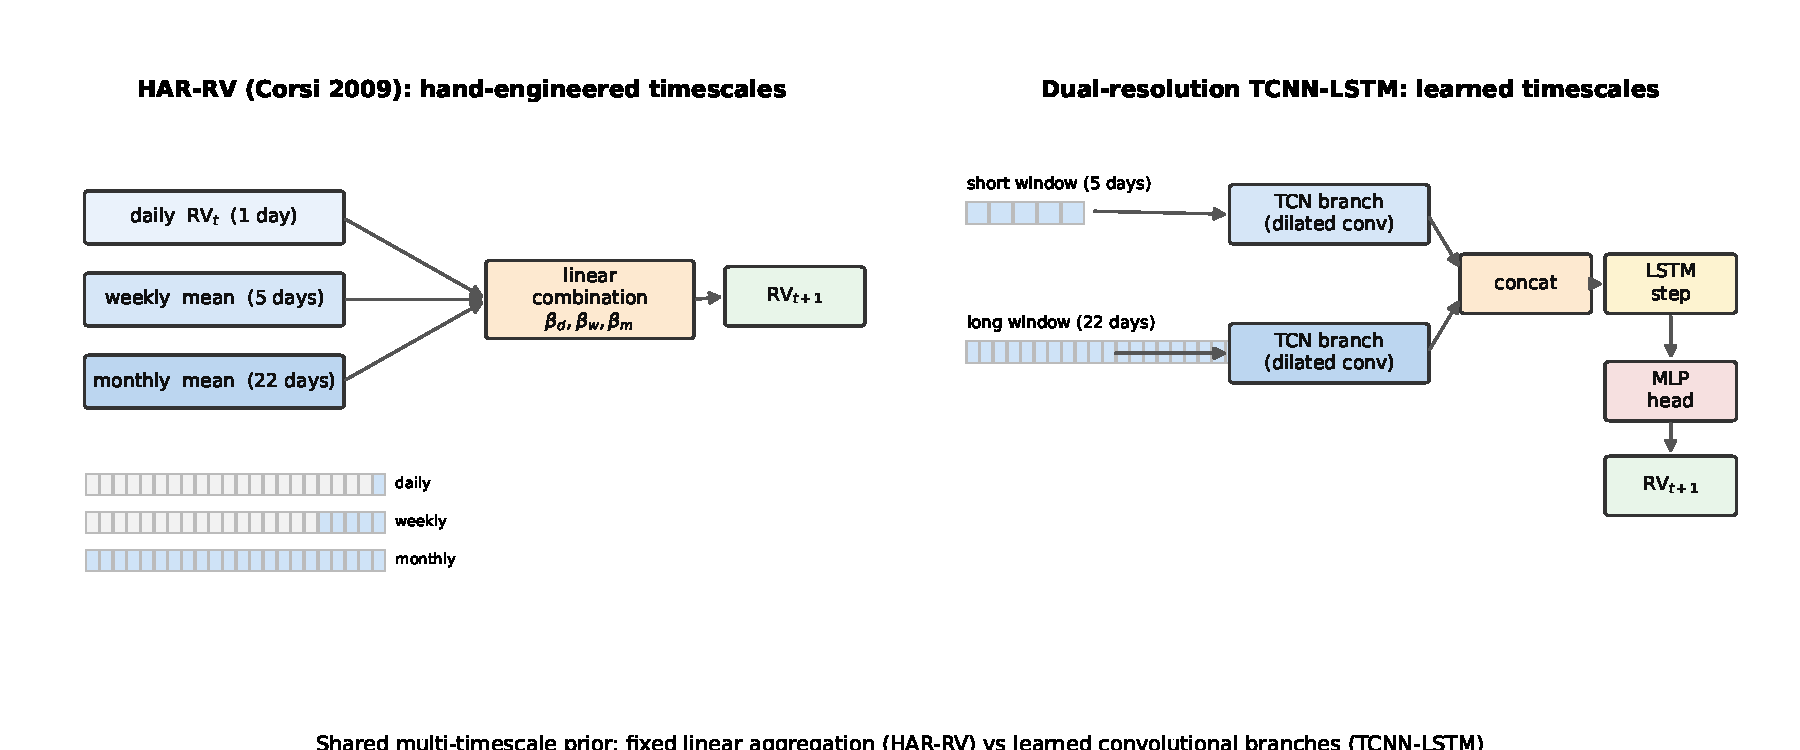
\includegraphics[width=\textwidth]{fig_har_analogy.pdf}
\caption{The shared multi-timescale prior. HAR-RV (left) combines fixed daily, weekly, and monthly
aggregates linearly; the dual-resolution TCNN-LSTM (right) learns convolutional features over a short
and a long window before fusing them. The transfer holds the information set equal and replaces the
fixed linear aggregation with a learned nonlinear one.}
\label{fig:analogy}
\end{figure}

\section{Proposed Method}
\textbf{Forecasting target.} All models forecast next-day log realized variance, $y_t=\log \mathrm{RV}_t$,
which stabilizes variance and approximate normality.

\textbf{Baselines.} HAR-RV regresses $y_{t+1}$ on $y_t$, the trailing five-day mean, and the trailing
22-day mean by ordinary least squares. GARCH(1,1) is fitted on daily returns; because it models
close-to-close return variance rather than the intraday range proxy used as the target, its
conditional-variance forecasts are aligned to the proxy level by a single additive constant in log
space estimated \emph{only} on the training set, which removes a definitional level offset without
using any validation or test information.

\textbf{Transferred model.} The dual-resolution TCNN-LSTM consumes a short window of five trading days
and a long window of 22 trading days, chosen so the combined information set matches HAR-RV's
daily-to-monthly span. Each window is processed by a stack of dilated 1-D convolutions (kernel 3,
dilations 1, 2, 4) followed by global average pooling; the two pooled feature vectors are concatenated
and passed as a length-one sequence through a single LSTM step and a small MLP head that emits the
scalar forecast. This mirrors the published HAR model \citep{warnants2026}, with the input reduced to a
single channel (univariate log-RV) and the objective changed from classification to mean-squared-error
regression. The network has 89{,}153 parameters and is trained with Adam (learning rate $10^{-3}$,
cosine schedule), batch size 64, and early stopping on validation RMSE.

\section{Data and Implementation}
The Oxford-Man Institute Realized Library, the standard source of 5-minute realized variance, was
discontinued in 2022, so we construct a daily realized-variance proxy from S\&P~500 index OHLC data
retrieved through Yahoo Finance (2000--2026). For each day we compute the Garman-Klass range-based
variance estimator \citep{garmanklass1980} and model its logarithm. The sample is split chronologically
into training (2000--2018, 4779 days), validation (2019--2020, 505 days), and test (2021--2025, 1255
days), with the validation window deliberately spanning the COVID-19 shock as an out-of-sample stress
test. The log-RV series shows the canonical features of volatility (Figure \ref{fig:data}): pronounced
clustering around 2008 and 2020, mild positive skew, and a slowly decaying autocorrelation function with
a partial autocorrelation that cuts off after roughly two lags, the long-memory signature that motivates
the HAR decomposition. We emphasize that the target is a daily \emph{range-based proxy}, not an intraday
realized measure, which has direct consequences for the achievable accuracy (Section \ref{sec:disc}).

\begin{figure}[H]
\centering
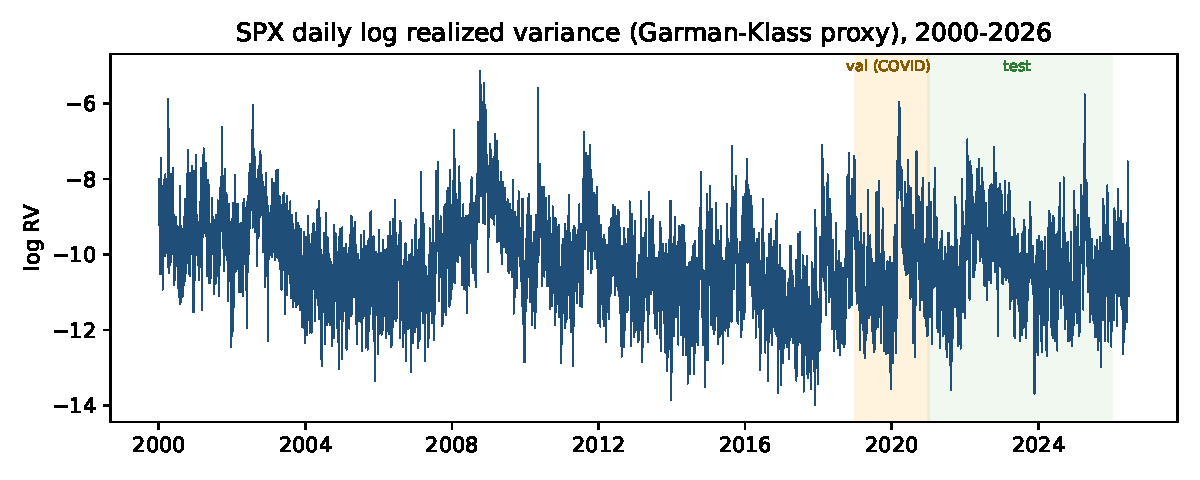
\includegraphics[width=0.49\textwidth]{fig_spx_logrv.pdf}\hfill
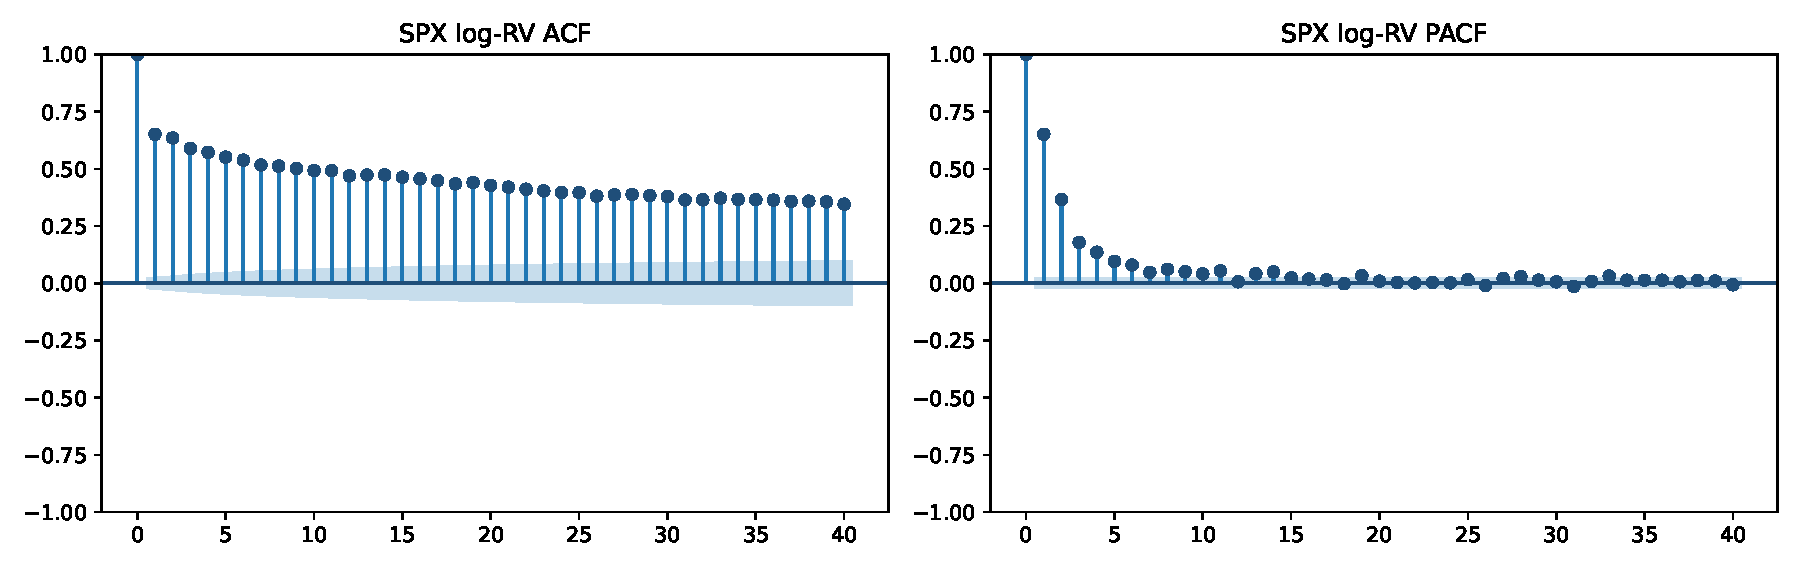
\includegraphics[width=0.49\textwidth]{fig_acf_pacf.pdf}
\caption{SPX daily log realized variance (left; validation and test windows shaded) and its
autocorrelation and partial autocorrelation (right). The slow ACF decay with a sharp PACF cutoff is the
long-memory signature underlying HAR-RV.}
\label{fig:data}
\end{figure}

All experiments are tracked with MLflow on a SQLite backend, with seeds fixed and logged. The stack is
Python 3.13 with PyTorch \citep{paszke2019pytorch} for the neural model, the \texttt{arch} package for
GARCH, and \texttt{statsmodels} for HAR-RV. The full environment is pinned and the pipeline is
regenerable from a single entry point; code is available in the project repository (see Appendix).

\section{Results}
Table \ref{tab:metrics} reports forecast accuracy. On the test set the transferred TCNN-LSTM attains the
lowest squared-error loss (log-RMSE 0.823) ahead of HAR-RV (0.835) and GARCH (0.884). Diebold-Mariano
tests \citep{dieboldmariano1995} with the small-sample correction of \citet{harvey1997} confirm the
ordering under squared-error loss is statistically significant (Table \ref{tab:dm}): the TCNN-LSTM
improves on HAR-RV ($p=0.013$) and on GARCH ($p<0.001$), and HAR-RV improves on GARCH ($p<0.001$).
Figure \ref{fig:pred} shows that all models track the test-period dynamics, with the deep model
following the peaks slightly more closely.

\begin{table}[H]
\centering
\caption{Forecast accuracy on SPX. RMSE is on log-RV; QLIKE \citep{patton2011} is on RV. Lower is better;
best test values in bold.}
\label{tab:metrics}
\begin{tabular}{lcccc}
\toprule
Model & Val log-RMSE & Val QLIKE & Test log-RMSE & Test QLIKE \\
\midrule
GARCH(1,1) & 0.947 & 0.457 & 0.884 & 0.454 \\
HAR-RV     & 0.896 & 0.515 & 0.835 & 0.445 \\
TCNN-LSTM  & 0.879 & 0.471 & \textbf{0.823} & \textbf{0.424} \\
\bottomrule
\end{tabular}
\end{table}

\begin{table}[H]
\centering
\caption{Pairwise Diebold-Mariano tests on the test set (negative statistic favors the first model). The
RMSE improvements are significant; under QLIKE only the HAR-RV vs TCNN-LSTM pair is significant.}
\label{tab:dm}
\begin{tabular}{lcccc}
\toprule
Pair & SE stat & SE $p$ & QLIKE stat & QLIKE $p$ \\
\midrule
GARCH vs HAR-RV     & $+4.71$ & 0.000 & $+0.47$ & 0.638 \\
GARCH vs TCNN-LSTM  & $+5.38$ & 0.000 & $+1.27$ & 0.203 \\
HAR-RV vs TCNN-LSTM & $+2.49$ & 0.013 & $+2.17$ & 0.030 \\
\bottomrule
\end{tabular}
\end{table}

\begin{figure}[H]
\centering
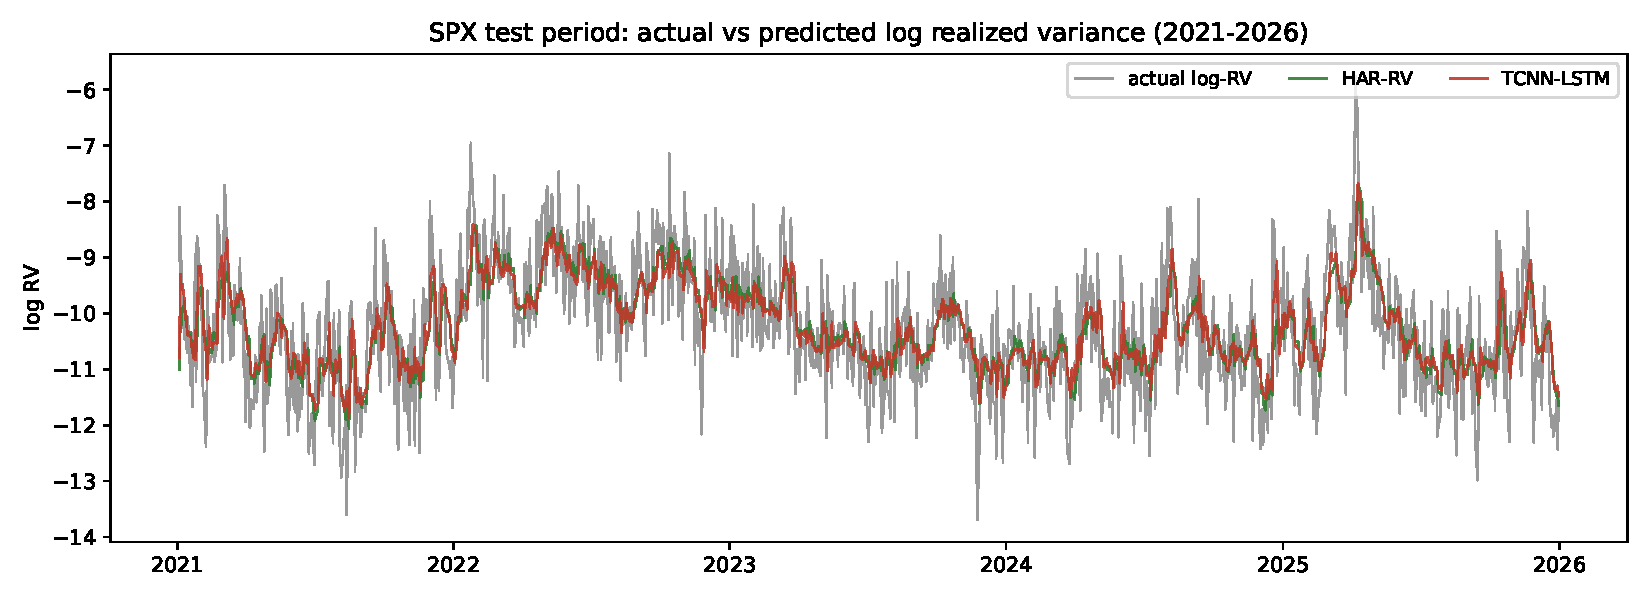
\includegraphics[width=\textwidth]{fig_predictions.pdf}
\caption{Actual versus predicted log realized variance over the SPX test period (2021--2026).}
\label{fig:pred}
\end{figure}

\textbf{Robustness and ablation.} Because the headline comparison used a single random seed, we trained
the model under five seeds and ran a branch ablation (Figure \ref{fig:robust}). The squared-error
improvement is robust: all five seeds beat HAR-RV with a test log-RMSE of $0.824\pm0.002$. The QLIKE
advantage is not robust; only one of five seeds beats HAR-RV on QLIKE, so we report the squared-error
result as the finding and treat the seed-42 QLIKE win as indicative only. The ablation shows the
dual-resolution design contributes: removing the short branch raises test RMSE to 0.827 and removing the
long branch to 0.830, so both timescales carry signal, with recent history dominant.

\begin{figure}[H]
\centering
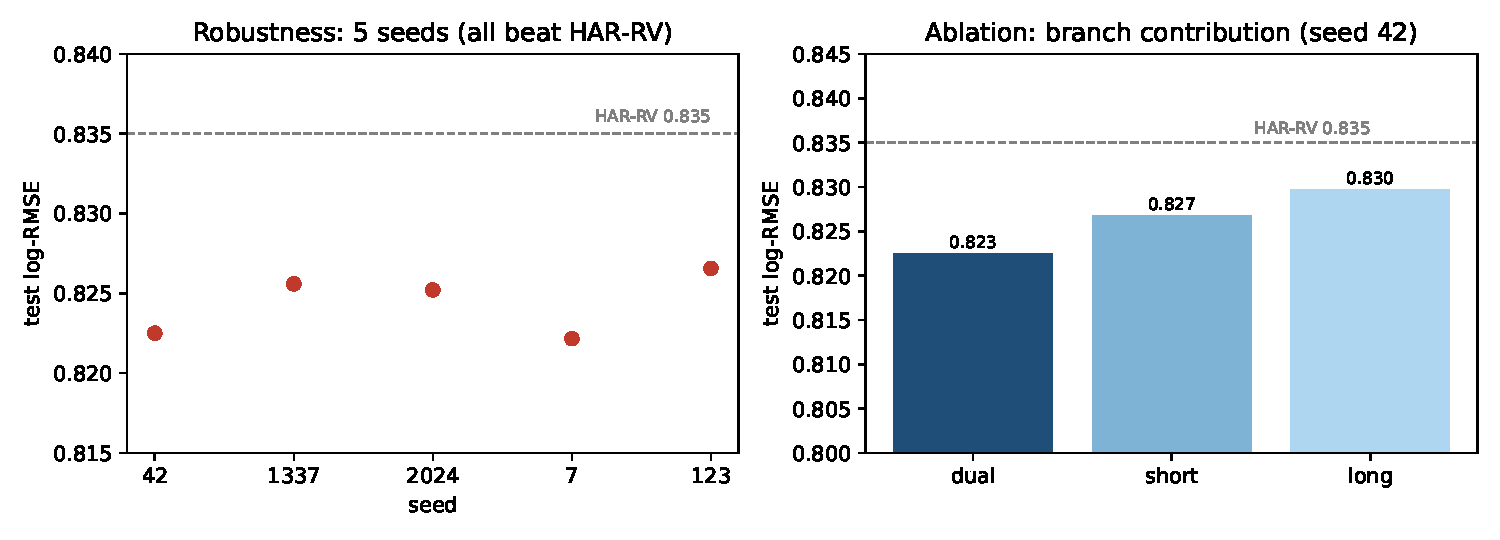
\includegraphics[width=\textwidth]{fig_robustness_ablation.pdf}
\caption{Left: five-seed robustness; every seed beats HAR-RV on test RMSE. Right: branch ablation; the
dual model outperforms either single branch.}
\label{fig:robust}
\end{figure}

\section{Discussion and Limitations}
\label{sec:disc}
The transfer succeeds in a measurable but modest way: replacing HAR-RV's fixed linear aggregation with
learned convolutional branches over the same information set yields a small, robust, and statistically
significant reduction in squared forecast error, while leaving variance-space (QLIKE) loss essentially
unchanged. Three limitations frame this result honestly. First, the absolute RMSE of every model is high
relative to the realized-volatility literature because our target is a daily Garman-Klass proxy rather
than a 5-minute realized measure; this measurement noise is irreducible and bounds the achievable error
for all models equally, so only the relative comparison is informative, and it likely compresses the gap
between a linear and a nonlinear model. Second, the study covers a single asset (SPX) and a single
architecture trained once per seed; broader cross-sectional and multi-architecture evidence would
strengthen the claim. Third, the GARCH level calibration, while estimated only on training data, is a
modeling choice that a stricter evaluation might replace with a model matched to the same proxy.

The most useful reading of the result is about where the multi-timescale prior pays off. At the daily
horizon with a noisy proxy, Corsi's linear decomposition is already near-optimal, so the learned model
gains little. The architecture's value in the HAR domain came from genuinely nonlinear interactions
among sensor channels; financial volatility at this horizon may simply not contain enough nonlinearity to
reward the inductive bias. This points to intraday horizons, regime-switching periods, and multi-asset
cross-sections, where nonlinearity is stronger, as the more promising settings for the transfer.

\section{Conclusion}
We transferred a dual-resolution hybrid TCNN-LSTM from human activity recognition to daily volatility
forecasting, motivated by the structural identity between its short-and-long-context design and HAR-RV's
multi-timescale decomposition. On SPX the transferred model significantly and robustly improves on HAR-RV
and GARCH under squared-error loss, with the improvement validated across seeds and attributed to the
dual-resolution structure by ablation, while being honestly bounded by the noise of the daily proxy. The
contribution is a clean, testable bridge from a known financial inductive bias to a learned architecture
that respects it.

\bibliographystyle{plainnat}
\bibliography{refs}

\appendix
\section{Hyperparameters and Fitted Coefficients}
TCNN-LSTM: short window 5, long window 22, TCN channels (32, 64), dilations (1, 2, 4), LSTM hidden 64,
dropout 0.1, Adam lr $10^{-3}$ with cosine schedule, batch 64, max 200 epochs, early stopping patience
15, seed 42; 89{,}153 parameters; best epoch 27. HAR-RV coefficients (SPX): const $-0.678$, daily 0.149,
weekly 0.462, monthly 0.323 (slopes sum 0.933, reproducing Corsi's near-unit persistence). GARCH(1,1):
$\mu=0.062$, $\omega=0.025$, $\alpha=0.120$, $\beta=0.861$ (persistence 0.981), log-level calibration
offset $-0.870$.

\section{Reproducibility and Code}
All runs are logged to MLflow with fixed seeds. The repository contains the data pipeline, models,
training loop, evaluation, and the robustness and ablation drivers, regenerable end to end.
Repository: \url{https://github.com/MohamedJJ824/volatility-project}.

\section{Training Curve}
\begin{figure}[H]
\centering
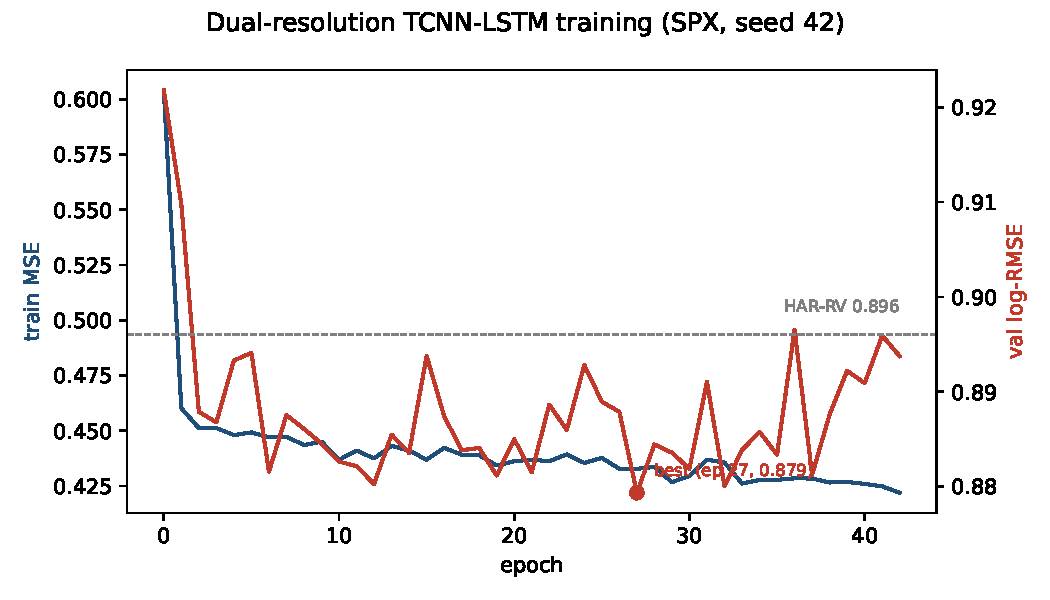
\includegraphics[width=0.7\textwidth]{fig_training_curves.pdf}
\caption{TCNN-LSTM training: train MSE and validation log-RMSE per epoch, with the early-stopped best
epoch and the HAR-RV reference marked.}
\label{fig:train}
\end{figure}

\section{Use of AI Tools}
Claude Code (claude-opus-4-8) was used as a coding and writing assistant throughout, under the course
policy permitting AI coding tools with disclosure. It was used to scaffold the data pipeline, the
GARCH/HAR-RV baselines, the TCNN-LSTM and training loop, the Diebold-Mariano test, the figures, and a
draft of this report. All outputs were verified by the author: model coefficients were checked against
known regularities (HAR slopes positive and summing near one; GARCH persistence near 0.98), the RMSE
floor was confirmed by benchmarking against climatology and a random walk, the significant single-seed
result was re-tested across five seeds, and every figure and number was inspected before inclusion. A
cumulative tool-usage log is maintained in the repository.

\end{document}
